
GIM alebo Glucose-Insulin Model softvér nám dáva schopnosť simulovať chovanie sa jedinca a jeho sekréciu inzulínu.\cite{2007}

V poslednej dobe bol navrhnutý nový model simulácie jedla, ktorý umožnil meranie rôznych tokov, glukózy a inzulínu, vyskitujúcich sa počas jedla. V skutočnosti je systém, veľmi zložitý a iba dostupnosť tokov glukózy a inzulínu, ich plazmatických koncentrácií, nám umožní minimalizovať štruktúrne neistoty pri modelovaní rôznych procesov. Model pozostáva z 12 nelineárnych diferenciálnych rovníc, 18 algebraitických rovníc a 35 parametrov.\cite{2007}

Užívateľsky príjemný simulačný softvér tohto modelu by bol veľkou pomocou, najmä pre vyšetrovateľov bez konkrétnych odborných znalostí v oblasti modelovania.Softvér GIM, implementovaný v MATLAB verzii 7.0.1, ktorý umožňuje simulovať normálne aj patologické stavy, napr. Diabetes typu 2 a inzulín s otvorenou a uzavretou slučkou infúzie pri cukrovke 1. typu. Softvér sa nepokúša riešiť patofyziologické otázky.\cite{2007}

\subsection{MATLAB Version}

Keď je GIM spustený, otvorí sa dialógové okno\ref{okno1}, ktoré čaká od užifvateľa, aby zvolil typ subjektu pre modelovanie. Na výber sú tri možnosti, a to Normálny, typ 2 Diabetik aleb o typ 1 Diabetik.

\begin{figure}[H]
\centering
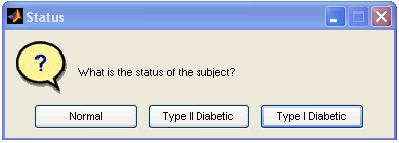
\includegraphics[scale=1]{ob-1.PNG}
\caption{dialógové okno - 1 \cite{2007}}
\label{okno1}
\end{figure}

Keď používateľ klikne na subjekt Normálny alebo Diabetik 2. typu, zobrazí sa interaktívne okno\ref{okno2}, ktoré je rozdelené na tri časti. 

1. Bazálne, kde sú stanovené základné hodnoty koncentrácie glukózy, koncentrácie inzulínu a produkcie glukózy. Kliknutím na tlačidlo VÝPOČET sa vypočíta bazálna hodnota glukózy a zobrazí sa na príslušnom štvorci \cite{2007}

2. Subjekt, kde sú hodnoty telesnej hmotnosti a hlavné metabolické indexy, ako sú periférna a hepatálna citlivosť na inzulín (Vmax a kp3, v tomto poradí), dynamická a statická odozva beta-buniek na glukózu (K a beta, v tomto poradí ), sa zadávajú ako percento bežných hodnôt12; pre diabetické subjekty typu 2 sa spočiatku zobrazia typické odchýlky. \cite{2007}

3. Protokol, kde je nastavený čas troch jedál a množstvo prijatej glukózy. \cite{2007}

\begin{figure}[H]
\centering
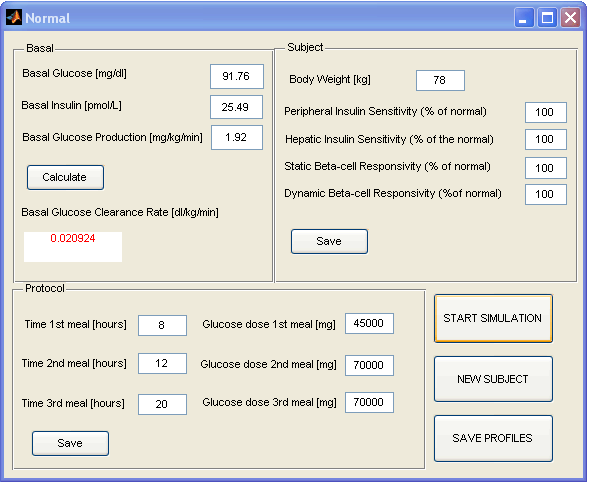
\includegraphics[scale=0.8]{ob-2.PNG}
\caption{dialógové okno - 2 \cite{2007}}
\label{okno2}
\end{figure}

Akonáhle sú všetky polia nastavené a nové hodnoty sú uložené, simulácia sa spustí kliknutím na START SIMULATION. Výsledky simulácie sú prezentované v grafickom formáte \ref{okno3}, tj. Je zobrazený obrázok, ktorý ukazuje koncentrácie glukózy a inzulínu, produkciu glukózy, využitie glukózy, vzhľad jedla a sekréciu inzulínu.\cite{2007}

\begin{figure}[H]
\centering
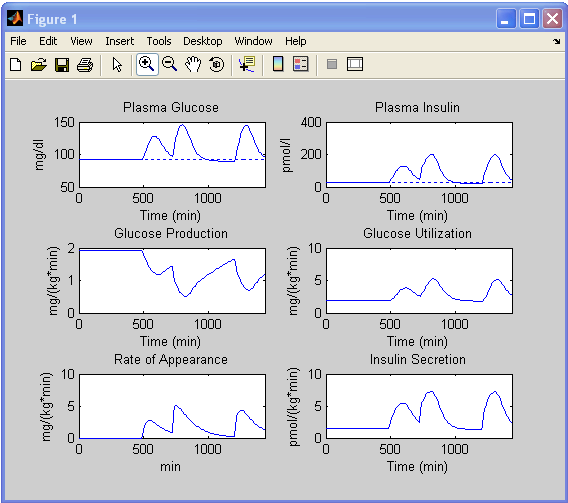
\includegraphics[scale=0.8]{ob-3.PNG}
\caption{dialógové okno - 3 \cite{2007}}
\label{okno3}
\end{figure}

Keď požívateľ zvolí  Diabtik 1. typu, okno je o trochu inšie, pridá sa tam jedna sekcia\ref{okno4}.

4. Kontrola, ktorá umožňuje užívateľovi vybrať, či je subjekt kontrolovaný v otvorenej slučke alebo v uzavretej slučke s regulátorom PID. Ak je zvolená otvorená slučka, je možné zadať rýchlosť infúzie bazálneho inzulínu. Ak je zvolená uzavretá slučka, užívateľ môže zvoliť bazálnu koncentráciu inzulínu, ktorý musí tiež definovať cieľovú hodnotu glukózy. \cite{2007}

\begin{figure}[H]
\centering
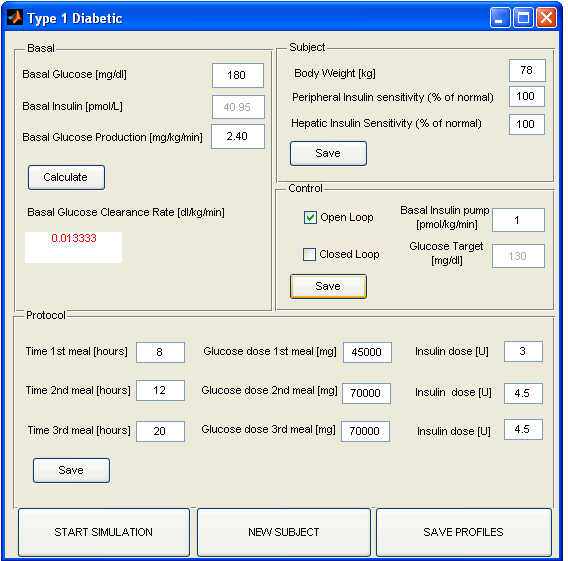
\includegraphics[scale=0.8]{ob-4.PNG}
\caption{dialógové okno - 3 \cite{2007}}
\label{okno4}
\end{figure}

Program taktiež umožňuje ukladať si profily a výsledky v .mat typoch súborov, stalčením SAVE PROFILES.\cite{2007}

Softvér GIM umožňuje taktiež porovnávanie výsledkov medzi normálnym, zdravím jedincom a Diabetikom 1. typu, poprípade rôznej kombinácii 2 subjektov.\cite{2007}

\paragraph{Grafické vyjadrenie informácií v informatike}
Viete v informatike, keď sa pripravuje nejaký softvér treba dbať aj na konečného užívateľa. Dobrým príkladom môže byť GIM. Jeho prostredie väčšine laikom povie akurát tak nič. Treba mať presne zadefinované, kto bude daný softvér používať. V prípade GIM simulátora sú to lekári a laboratórny pracovníci. Ak si vezmeme iný, voľne dostupný softvér pre diabetikov, je omnoho ústretovejší a prehľadnejší pre laikov, bežných ľudí.